% English version of paper/ja_v2/04_問い1a.md (2026-11-17).
\section{RQ1(a): answer bias was almost removed without labels, and the remaining error was reduced by pseudo-labels from classifiers including other modalities}\label{sec:rq1a}

RQ1(a) asks which part of the linear classifier's error each of the four information sources corrects. With one source corpus, audio and visual answer bias was almost removed both by correcting intercepts with the K labels and by label-free feature-mean subtraction. The separation of target-only classifiers stayed below $D^{*}$ (defined in Sect.~\ref{sec:twoerrors}) for audio and text even at K = 25 (0.77 and 0.58 of $D^{*}$), and with all other groups as sources it was rarely reduced by eight methods using same-modality unlabelled utterances and was reduced by pseudo-labels from classifiers including other modalities.

\subsection{Setting}

\subsubsection{Two parts of the error}\label{sec:twoerrors}
A linear classifier assigns an emotion using, for each pair of emotions, a boundary in feature space whose direction is set by the weights and whose position is set by the intercepts (Fig.~\ref{fig:twoerrors}). An error in which the boundary has the right direction but is shifted, so that predictions are biased towards one emotion, is the \emph{answer bias}; it disappears when only the intercepts are corrected. The error that remains after correcting the bias is the \emph{remaining error}; it shrinks only when the direction of the weights changes. Answer bias and remaining error are defined conceptually; we quantify them by the intercept loss and the direction loss defined below.

\begin{figure}[t]
\centering
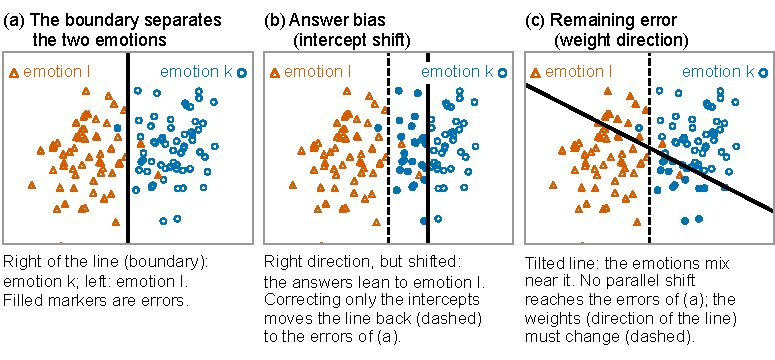
\includegraphics[width=\textwidth]{figures/fig_two_errors_en.pdf}
\caption{Two parts of the error of a linear classifier, drawn in a two-dimensional feature space. (a) The boundary separates the two emotions. (b) Answer bias: the direction is right but the boundary is shifted, biasing predictions towards one emotion; correcting only the intercept returns to (a). (c) Remaining error: the boundary is tilted, and no parallel shift brings the errors down to those of (a). The points are illustrative, not experimental data}\label{fig:twoerrors}
\end{figure}

For the score $s_k(x)=w_k^\top x+b_k$ of emotion $k$, the decision between emotions $k$ and $l$ is the sign of $z_{kl}=(w_k-w_l)^\top x+(b_k-b_l)$. With mean $\hat\mu_k$ and variance $v_k$ of $z_{kl}$ over target test utterances of emotion $k$ (likewise for $l$) and $\sigma=\sqrt{(v_k+v_l)/2}$, we define
\begin{equation}
d_{kl}=\frac{\hat\mu_k-\hat\mu_l}{\sigma},\qquad o_{kl}=-\frac{\hat\mu_k+\hat\mu_l}{2\sigma},
\end{equation}
the separation of the two emotions on the decision axis and the offset of the boundary ($z_{kl}=0$) from the midpoint of their means. If $z_{kl}$ of both emotions is normal with equal variance, the pairwise accuracy is $A(d,o)=\tfrac12[\Phi(d/2-o)+\Phi(d/2+o)]$. With the separation $D^{*}$ along the linear discriminant direction of the labelled target utterances (Ledoit--Wolf shrinkage \cite{ledoit2004}), the pairwise loss splits as
\begin{equation}
A(D^{*},0)-A(d,o)=\underbrace{[A(D^{*},0)-A(d,0)]}_{\text{direction loss}}+\underbrace{[A(d,0)-A(d,o)]}_{\text{intercept loss}}.
\end{equation}
Changing only the intercepts shifts $z_{kl}$ equally for all utterances and moves only $o$; a shift $x\to x+\delta$ common to all emotions also moves only $o$, so subtracting each corpus's feature mean does not change the direction loss. $D^{*}$ is used only for evaluation and is not the largest separation over linear directions. When this equal-variance Gaussian approximation was checked on source-only classifiers of the single-source setting, the median approximation error was 0.41--1.27 times the median intercept loss, failing the pre-set criterion (below 1/3), so answer bias is measured by UAR differences rather than by the approximation. For the direction loss the ratio was 0.05--0.13, meeting the criterion except for visual features (0.47).

\subsubsection{Single-source setting}\label{sec:rq1a-single}
We compare at K = 5 on the test utterances the merged classifier (all utterances of one source group and the K target labels; $C$ fixed to that of the source-only classifier), the source-only classifier, the target-only classifier (K labels only), an \emph{intercept-only fix} (weights of the source-only classifier fixed, four intercept shifts learned on the K labels) and \emph{mean subtraction} (each corpus's mean over all its utterances, including target test utterances, subtracted before retraining; no target labels). Neither of the last two changes the direction loss, so the ratio of their gain (method $-$ source-only) to the merged gain (merged $-$ source-only) measures how much of the merged gain correcting answer bias alone obtains. The remaining error is measured by how close the separation $d_T(K)$ of the target-only classifier comes to $D^{*}$ ($d_T/D^{*}$). Intervals are percentile intervals of a two-stage bootstrap over speakers (clusters for MOSEI) and repetitions; for targets with fewer than 20 effective speakers, the union of this interval and a speaker-jackknife $t$ interval is used.

\subsubsection{All-source setting}\label{sec:rq1a-all}
Against the K-label baseline retrained from the anchor of all non-target groups, we measure whether two kinds of methods reduce the direction loss averaged over the six emotion pairs. Hyperparameters are chosen with each source group as a provisional target, and intervals are two-stage bootstrap percentile intervals over speakers and repetitions, with the same resamples applied to a method and the baseline.
\begin{itemize}
\item \textbf{Distillation:} a cross-entropy term towards the pseudo-labels of unlabelled utterances is added to the loss of the K-label baseline. In this setting the provider and weighting of the pseudo-labels were chosen per condition on provisional targets (mostly the product of the classifiers' probabilities; audio and visual only when the modalities are audio and visual), and all include the retrained classifier's own modality. Measured in 81 conditions (each classifier with audio, visual and text on three corpora and with audio and visual on five corpora; K = 0, 5, 25).
\item \textbf{Eight methods using same-modality unlabelled utterances:} entropy minimisation, self-training, information maximisation (IM) \cite{liang2020,boudiaf2020}, test-time template adjuster (T3A) \cite{iwasawa2021}, label propagation, CORAL, DANN and MME; single modality, K = 0, 5; 210 conditions.
\end{itemize}
The two counts come from different sets of conditions. Verdicts follow pre-set rules: a method \emph{reduced} the direction loss if the 95\% interval of (baseline $-$ method) was above zero and the point estimate at least $\delta$, \emph{increased} it if below zero and at most $-\delta$, was at the \emph{same level} if the interval lay within $\pm\delta$, and was \emph{undetermined} otherwise; $\delta$ (0.82--1.11\pt\ for the 81 conditions, 0.89--1.10\pt\ for the 210) was set from provisional-target outputs only. Some pseudo-label options (such as the product) were added after seeing results of an earlier version of the method on the same corpora.

\subsection{Results}

\subsubsection{Mixing in a source corpus helped at K = 1 and hurt with all target labels}
The gain of the merged classifier over the target-only classifier was positive for all eight feature sets at K = 1 (from 6.9\pt\ [4.8, 8.7] for V to 13.4\pt\ [11.4, 15.4] for AV), decreased with K, and was negative for all eight with all target training labels (from $-$2.1\pt\ for V to $-$4.8\pt\ for T; all intervals below zero).

\subsubsection{Answer bias was almost corrected by intercepts or by mean subtraction}
Table~\ref{tab:bias} shows that, for audio and visual features, the intercept-only fix and mean subtraction obtained most of the merged gain (merged $-$ source-only). The summed intercept-only gain divided by the summed merged gain was 0.91 for audio (WavLM), 0.90 for audio (HuBERT) and 0.78 for visual. Mean subtraction gained 4.69\pt\ [3.81, 5.57] for audio (WavLM) against the merged 5.26\pt, and 2.40\pt\ for visual against 2.47\pt. Correcting intercepts on the K labels after mean subtraction did not give an interval above zero for any of the eight feature sets.

\begin{table}[t]
\caption{Single-source setting, K = 5: UAR differences in points on test utterances. ``Ratio'' is $\sum$(intercept-only $-$ source-only) $/ \sum$(merged $-$ source-only) over pairs; the last column is relative to mean subtraction, with 95\% intervals. Values are pair means (each pair averaged over repetitions 0--9)}\label{tab:bias}
\footnotesize\setlength{\tabcolsep}{4pt}
\begin{tabular}{@{}lrrrl@{}}
\toprule
 & Merged $-$ & Mean sub.\ $-$ & & Mean sub.\ + intercepts \\
Features & source-only & source-only & Ratio & $-$ mean sub. \\
\midrule
Audio (WavLM) & +5.26 & +4.69 & 0.91 & +0.38 [$-$0.12, +0.88] \\
Audio (HuBERT) & +4.73 & +4.18 & 0.90 & +0.18 [$-$0.42, +0.77] \\
Visual & +2.47 & +2.40 & 0.78 & $-$0.39 [$-$0.78, +0.02] \\
\botrule
\end{tabular}
\end{table}

\subsubsection{Target-only classifiers reached 0.77 (audio) and 0.58 (text) of $D^{*}$ at K = 25}
The ratio $d_T/D^{*}$ of target-only classifiers (median over targets of the ratio averaged over six emotion pairs) was 0.23, 0.47, 0.62 and 0.77 for audio (WavLM) at K = 1, 5, 10 and 25, and 0.11, 0.32, 0.42 and 0.58 for text. Visual reached 1.01 at K = 10 (1.10 at K = 25; the ratio can exceed 1 because $D^{*}$ is not the largest linear separation). For audio and text, 25 labels per emotion did not raise the separation of target-only classifiers to $D^{*}$.

\subsubsection{With all groups as sources, pseudo-labels from classifiers including other modalities reduced the remaining error}
Table~\ref{tab:allsource} shows that distillation reduced the direction loss in 38 of 81 conditions and increased it in one; its UAR was judged higher than the K-label baseline (same rule) in 32 and lower in none. The eight methods reduced the direction loss in 7 of 210 conditions and increased it in 79. If the true differences were zero and conditions independent, the expected numbers of ``reduced'' conditions would be 2.02 and 5.25. Comparing point estimates on the same anchors and conditions (two groups, K = 0 and 5), distillation reduced the direction loss more in 341 of 373 pairs (pairs are not independent).

\begin{table}[t]
\caption{All-source setting: numbers of conditions by verdict. Direction loss: reduced / same level / increased / undetermined; UAR (method $-$ K-label baseline): higher / same level / lower / undetermined. ``16 more'' are conditions in which the adaptation term of DANN or MME did not change predictions beyond seed variation (separate from the 48 undetermined). Visual direction losses come from features that failed the approximation check (Sect.~\ref{sec:twoerrors})}\label{tab:allsource}
\footnotesize
\begin{tabular}{@{}llrll@{}}
\toprule
Modalities & Classifier & Conditions & Direction loss$^{a}$ & UAR \\
\midrule
A, V, T (3 corpora) & Audio & 9 & 9/0/0/0 & 9/0/0/0 \\
 & Visual & 9 & 1/1/0/7 & 1/0/0/8 \\
 & Text & 9 & 5/0/1/3 & 4/0/0/5 \\
 & AVT & 9 & 6/1/0/2 & 5/2/0/2 \\
A, V (5 corpora) & Audio & 15 & 7/0/0/8 & 7/0/0/8 \\
 & Visual & 15 & 5/0/0/10 & 4/1/0/10 \\
 & AV & 15 & 5/5/0/5 & 2/2/0/11 \\
\midrule
Distillation, total & & 81 & 38/7/1/35 & 32/5/0/44 \\
Eight methods & A, V, T & 210 & 7/60/79/48 (16 more) & --- \\
\botrule
\end{tabular}
\footnotetext{$^{a}$Halving $\delta$ gives 49 of 81 ``reduced'' conditions for distillation; doubling it gives 20}
\end{table}

\subsection{Answer to RQ1(a)}
\begin{itemize}
\item \textbf{K target labels:} with one source corpus, they mainly corrected answer bias for audio and visual features (the intercept-only fix obtained 0.78--0.91 of the merged gain). The separation of target-only classifiers stayed at 0.77 (audio) and 0.58 (text) of $D^{*}$ even at K = 25.
\item \textbf{Unlabelled target utterances:} subtracting the feature mean almost corrected the bias (+4.69\pt\ for audio against the merged +5.26\pt); eight methods using same-modality unlabelled utterances reduced the remaining error in only 7 of 210 conditions.
\item \textbf{Labelled source utterances:} the gain of mixing was positive at K = 1 and negative with all target labels; most of the merged gain was also obtained by the intercept-only fix or mean subtraction, i.e., it mainly came from correcting answer bias.
\item \textbf{Pseudo-labels from classifiers including other modalities:} they reduced the remaining error in 38 of 81 conditions and lowered UAR in none.
\end{itemize}
Because audio and visual answer bias was almost removed without labels in the single-source setting, further UAR gains on a new corpus would have to come from reducing the remaining error, for which pseudo-labels from classifiers including other modalities were the information source that worked in the all-source setting. Section~\ref{sec:rq1b} therefore examines which classifiers distillation improves and when in the LOCO setting with three source corpora, and Sect.~\ref{sec:rq2} examines how the pseudo-labels are built. Which error the K labels correct in the LOCO setting was not measured (Sect.~\ref{sec:limitations}).
